\documentclass[10pt,twoside]{article}
\usepackage[utf8]{inputenc}
\usepackage{amsmath}
\usepackage{amsfonts}
\usepackage{amssymb}
\usepackage[spanish,es-noshorthands]{babel}
\usepackage[T1]{fontenc}
\usepackage{lmodern}
\usepackage{graphicx,hyperref}
\usepackage{tikz,pgf}
\usepackage{multicol}
\usepackage{subfig}
\usepackage[papersize={6.5in,8.5in},width=5.5in,height=7in]{geometry}
\usepackage{fancyhdr}
\pagestyle{fancy}
\fancyhead[LE]{
\includegraphics[height=12pt]{Images/logo-colegio.png} Probabilidad $11^{\circ}$}
\fancyhead[RE]{}
\fancyhead[RO]{\textit{Germ\'an Avenda\~no Ram\'irez, Lic. U.D., M.Sc. U.N.}}
\fancyhead[LO]{}

\author{Germ\'an Avenda\~no Ram\'irez, Lic. U.D., M.Sc. U.N.}
\title{\begin{minipage}{.2\textwidth}

\includegraphics[height=1.75cm]{Images/logo-colegio.png}\end{minipage}
\begin{minipage}{.55\textwidth}
\begin{center}
Taller 03, Introducción a la probabilidad\\
Probabilidad $11^{\circ}$
\end{center}
\end{minipage}\hfill
\begin{minipage}{.2\textwidth}
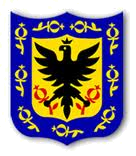
\includegraphics[height=1.75cm]{Images/logo-sed.png} 
\end{minipage}}
\date{}
\begin{document}
\maketitle
Nombre: \hrulefill Curso: \underline{\hspace*{44pt}} Fecha: \underline{\hspace*{2.5cm}}
\section*{Estad\'istica y los dulces}
De dónde vienen todos estos dulces tan coloridos?

¿Sabía usted que tienen 21 colores?

¿Sabía usted que la idea para los Dulces Sencillos de Chocolate “M\&M’s” nació
en el “telón de fondo” de la guerra civil española? Cuenta la leyenda que en un
viaje a España, Forrest Mars Sr. encontró soldados que comían bolitas de chocolate
cubiertas de una capa azucarada dura para evitar que se derritieran. Mr. Mars se
inspiró en este concepto y regresó a casa e inventó la receta para los Dulces Senci-
llos de Chocolate “M&M’s”.
La clase de estadística había comenzado y el maestro estaba hablando de por-
centajes, proporciones y probabilidad, y en qué forma son semejantes pero diferen-
tes. De pronto una estudiante dijo que escuchó que el grupo del semestre anterior
hizo una lección usando, y comiendo, chocolates M&M’s; ella preguntó si el grupo
de este año haría algo semejante. La conversación pronto se enfocó por entero en
los chocolates M&M’s, sus combinaciones de color y el porcentaje de cada color. A
los 24 miembros del grupo se les pidió que calcularan el porcentaje de cada color
que ellos pensaban estaba contenido en estas pequeñas bolsas de color café de los
Dulces Sencillos de Chocolate M&M’s. Se les dijo que habría un premio para la
persona cuyo cálculo fuera el más cercano al número real. Cada estudiante escri-
bió los porcentajes y los entregó; a su vez, los estudiantes recibieron una pequeña
bolsa café. “Ah, ¡esto es esa lección!”. “Sí” dijo el maestro, “y antes que abran esas
bolsas, debemos tener un plan”. Cada estudiante debía contar el número de choco-
lates M&M’s de cada color en su bolsa y anotar las seis cantidades; a continuación
podrían determinarse los totales del grupo. En la tabla 4.1 aparece la distribución
de cantidades resultante.
Los totales del grupo se convirtieron a porcentajes (tabla 4.2), y a cada estudian-
te se le pidió determinar los seis porcentajes que observaran en su propia bolsa de
chocolates M&M’s.
La discusión que siguió se centró en la variación que había de una bolsa a la
otra, con algunos estudiantes bastante sorprendidos de ver tanta variación. Varias
bolsas no tenían nada o sólo una pastilla de un color, y unas pocas bolsas tenían una
proporción más bien grande de sólo uno o dos colores. ¿Alguna vez había usted ob-
servado algunos de estos extremos cuando abría una bolsa de chocolates M&M’s?

\end{document}
